\documentclass[8pt,a5paper]{extarticle}
\usepackage[margin=1cm]{geometry}
\usepackage[utf8]{inputenc}
\usepackage[IL2]{fontenc}
\usepackage[czech]{babel}
\usepackage{microtype}
\usepackage{amssymb}
\usepackage{amsthm}
\usepackage{amsmath}
\usepackage{xcolor}
\usepackage{graphicx}

\usepackage[inline]{enumitem}

\newcommand{\R}{\mathbb{R}}

\setlist[enumerate]{label={(\alph*)},topsep=\smallskipamount,itemsep=\smallskipamount,parsep=0pt}
\setlist[itemize]{topsep=\smallskipamount,noitemsep}

\def\tisk{%
\newbox\shipouthackbox
\pdfpagewidth=2\pdfpagewidth
\let\oldshipout=\shipout
\def\shipout{\afterassignment\zdvojtmp \setbox\shipouthackbox=}%
\def\zdvojtmp{\aftergroup\zdvoj}%
\def\zdvoj{%
    \oldshipout\vbox{\hbox{%
        \copy\shipouthackbox
        \hskip\dimexpr .5\pdfpagewidth-\wd\shipouthackbox\relax
        \box\shipouthackbox
    }}%
}}%


\newtheorem*{poz}{Pozorování}

\theoremstyle{definition}
\newtheorem{uloha}{Úloha}
\newtheorem{suloha}[uloha]{\llap{$\star$ }Úloha}
\newtheorem*{bonus}{Bonus}
\newtheorem*{defn}{Definice}

\pagestyle{empty}

\let\=\doteq
\let\ee\expandafter

\def\vysld{}
\let\printvysl\relax
\let\printalphvysl\relax

\makeatletter
\def\vyslplain#1{\ee\ee\ee\gdef\ee\ee\ee\vysld\ee\ee\ee{\ee\vysld\ee\printvysl\ee{\the\c@uloha}{#1}}}

\def\locvysl#1{\ee\gdef\ee\locvysld\ee{\locvysld\item #1}}
\let\lv\locvysl

\newenvironment{ulohav}{\begin{uloha}\gdef\locvysld{\begin{enumerate*}}}{\ee\vyslplain\ee{\locvysld\end{enumerate*}}\end{uloha}}

\makeatother

\begin{document}

%\tisk

\section*{Kolmost a odchylky v prostoru}

Ve všech úlohách značí $S_{XY}$ střed úsečky $XY$.

\mathcode`\,="013B


\begin{ulohav}
Je dán pravidelný čtyřboký jehlan $ABCDV$, jehož stěny jsou rovnostranné trojúhelníky, $S$ je střed podstavy a $P$ střed hrany $AV$. Určete odchylky přímek
\begin{enumerate*}
    \item $BC$ a $SV$,\lv{$90^\circ$}
    \item $AB$ a $CV$,\lv{$60^\circ$}
    \item $AD$ a $CV$,\lv{$60^\circ$}
    \item $BV$ a $CP$,\lv{cca $77^\circ 5'$}
    \item $SV$ a $BP$.\lv{cca $65^\circ 54'$}
\end{enumerate*}
\end{ulohav}


\begin{ulohav}
V kvádru $ABCDEFGH$ s rozměry $|AB| = 6$, $|BC| = 3$, $|AE| = 8$ (kde $S$ je střed horní stěny a $M = S_{AE}$, $N = S_{BF}$) určete odchylky přímek
\begin{enumerate*}
    \item $BE$ a $CG$,\lv{$36^\circ 52'$}
    \item $EG$ a $BD$,\lv{$53^\circ 8'$}
    \item $AE$ a $BS$,\lv{$22^\circ 45'$}
    \item $BM$ a $NG$,\lv{$63^\circ 40'$}
    \item $AC$ a $BS$.\lv{$76^\circ 35'$}
\end{enumerate*}
\end{ulohav}


\begin{uloha}[Čistě rovinná]
Ve čtverci $ABCD$ jsme zvolili body $X$ na straně $CD$ a $Y$ na straně $AD$ tak, že $|CX| = |DY|$. Zdůvodněte, proč jsou na sebe úsečky $BX$ a $CY$ kolmé.
\[ 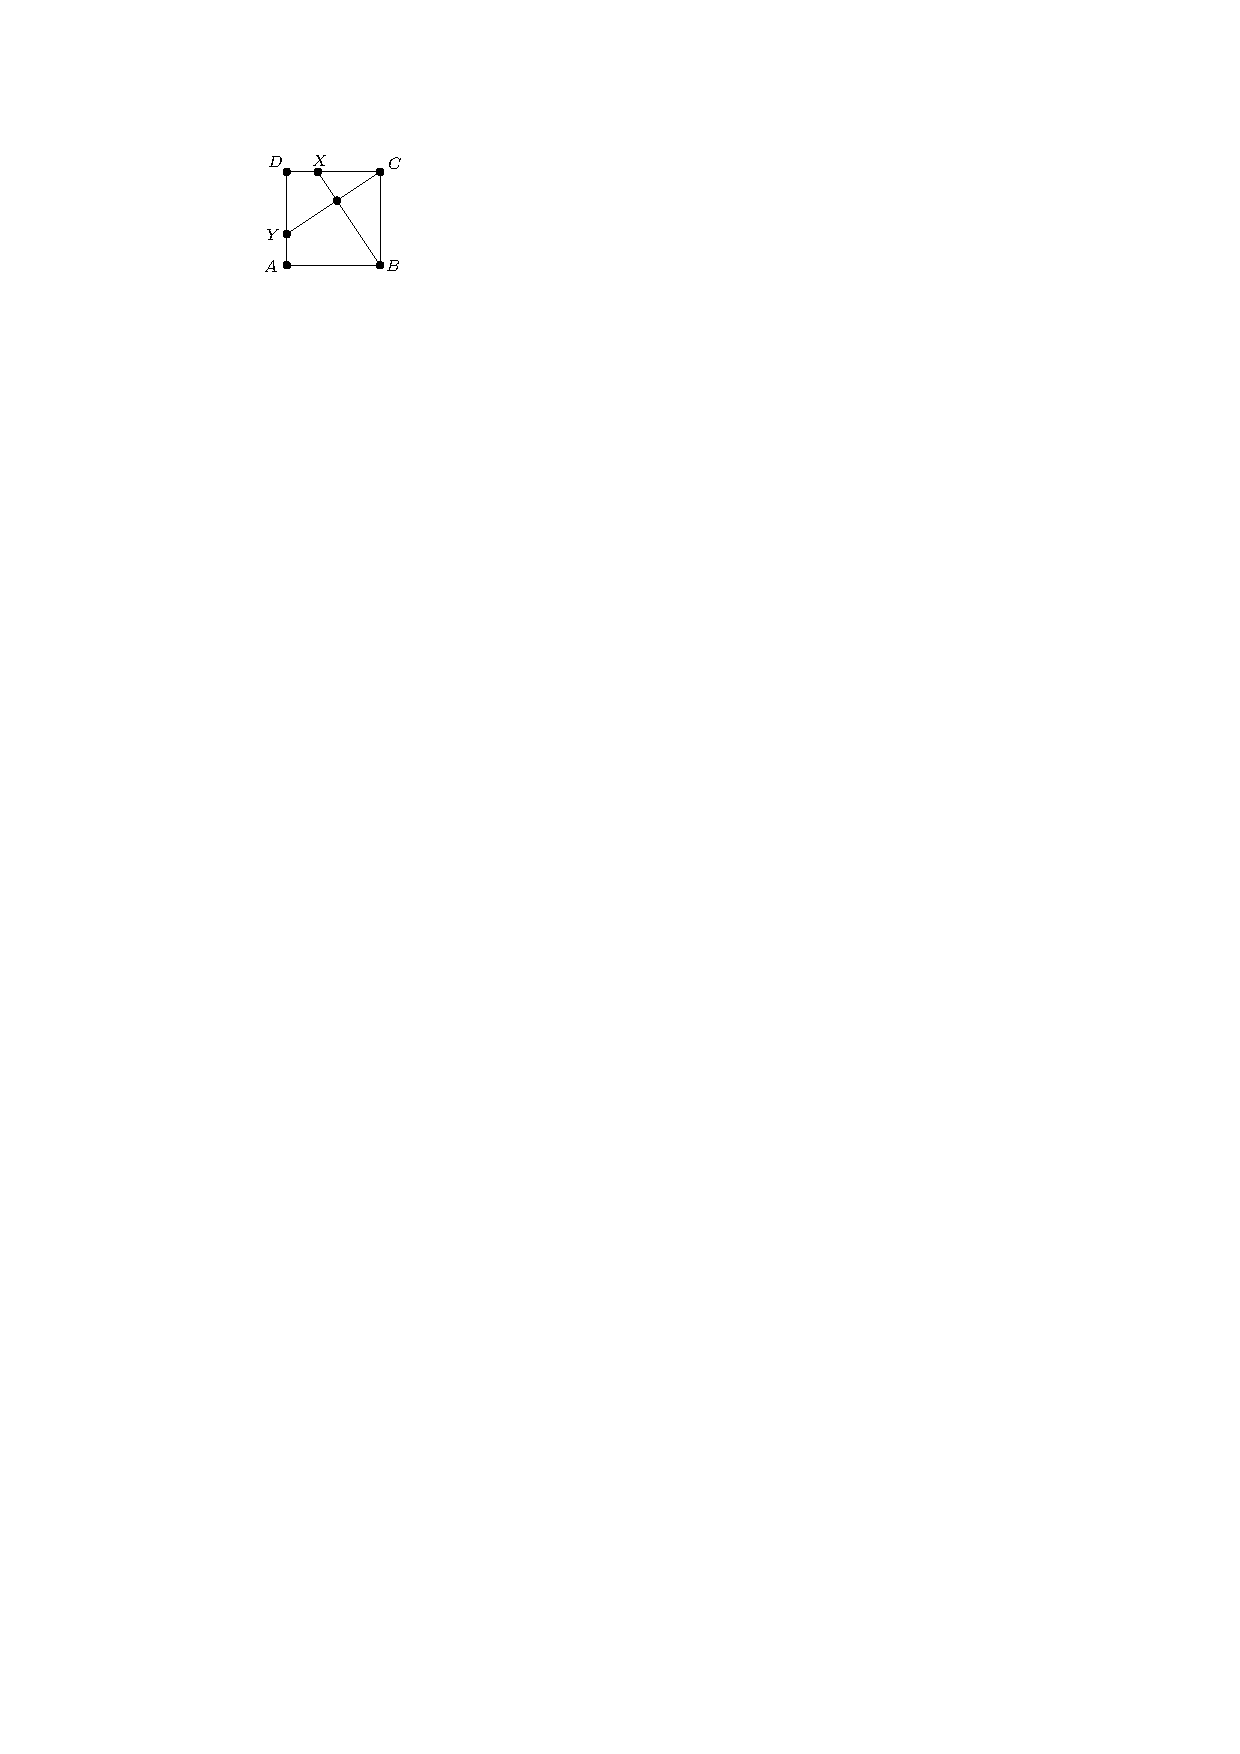
\includegraphics{ctverec_kolmost.pdf} \]
\end{uloha}

\begin{defn}
Řekneme, že přímka $p$ je kolmá k rovině $\varrho$, pokud je $p$ kolmá ke všem přímkám v~rovině $\varrho$. Značení: $p \perp \varrho$.
\end{defn}

\begin{poz}[Kritérium kolmosti přímky a roviny]
Je-li přímka $p$ kolmá ke dvěma různoběžným přímkám v~rovině $\varrho$, pak je $p$ kolmá k $\varrho$.
\end{poz}

\begin{uloha}
Pomocí Kritéria zdůvodněte, proč jsou na sebe kolmé následující dvojice přímek a rovin v krychli $ABCDEFGH$:
\begin{enumerate*}
    \item $EG$ a $BDH$,
    \item $BS_{FG}$ a $CDS_{BF}$,
    \item $AS_{CD}$ a $BFS_{EH}$,
    \item $FD$ a $ACH$.
\end{enumerate*}
\end{uloha}




\begin{uloha}
Rozmyslete si v krychli $ABCDEFGH$, co bude kolmým průmětem
\begin{enumerate*}
    \item bodů $E$ a $S_{AH}$ do roviny $BCG$,
    \item bodů $B$ a $S_{AB}$ do roviny $CDE$,
    \item bodu $S_{FG}$ do roviny $S_{AB}EH$,
    \item úsečky $AB$ do roviny $ACG$,
    \item bodu $F$ do roviny $ACH$.
\end{enumerate*}
\end{uloha}


\begin{suloha}
V krychli $ABCDEFGH$ zvolme body $X$, $Y$, $Z$ libovolně uvnitř stran $AB$, $AD$ a $AE$. Nechť $O$ je kolmý průmět $A$ do roviny $XYZ$.
\begin{enumerate*}
    \item Dokažte, že přímka $XO$ je kolmá na přímku $YZ$ (a podobně pro další dva body).
    \item Co je zač $O$ v trojúhelníku $XYZ$? Co jsme právě dokázali?
\end{enumerate*}
\end{suloha}


\begin{suloha}[Nijak nesouvisející s předchozím]
Uzavřená lomená čára, která sama sebe neprotíná, prochází všemi vrcholy určité krychle a láme se pouze v nich. Dokažte, že alespoň jeden segment oné čáry se shoduje s hranou oné krychle.
\end{suloha}


\newpage
\parindent=0pt
\parskip=\smallskipamount
\def\printvysl#1#2{\textbf{#1.}\ #2\par}
\vysld


\end{document}